

\section{Monte Carlo Algorithms}

Monte Carlo integration has been already extensively discussed in ICP (see \citep{comp_phys}). In this section, we will briefly summarize how this method works and go deeper into some details and properties we did not study in the past semester. 

\vspace{0.2cm}
\noindent
The basic idea behind Monte Carlo methods is that in order to calculate some thermodynamical quantity, it is enough to sample randomly in phase space instead of averaging over all states. If the sampling is large enough, the computed quantity will eventually converge toward the real thermodynamical quantity. The main steps in the Monte Carlo integration are:

\begin{itemize}
\item Choose randomly a new configuration in phase space (with a Markov chain).
\item Accept or reject the new configuration, depending on the strategy used (e.g., Glauber Dynamics).
\item Calculate the physical quantity and add it in the averaging loop.
\item Repeat the procedure.
\end{itemize}


\subsection{Markov Chains in Monte Carlo: M(RT)$^2$, Glauber, Kawasaki and Creutz algorithms}


\vspace{0.1cm}
\noindent
\begin{minipage}{\textwidth}
\begin{minipage}{.48\textwidth}
Often, choosing equally distributed configurations will be very inefficient since most of the possible configurations are unlikely to be assumed by the system. As an example take the kinetic energy of a gas. The distribution of the average energy will be a sharp peak, as in Fig. \ref{fig:sampling}. There are a number of methods to avoid unnecessary sampling of regions where the system is unlikely to be found (see \emph{importance sampling} in \citet{comp_phys} as an example).
\end{minipage}%
\hfill
\begin{minipage}{.48\textwidth}
  \centering
  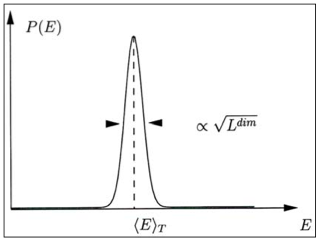
\includegraphics[height=150pt]{pics/sampling}
  \captionof{figure}{Example of energy distribution}
  \label{fig:sampling}
\end{minipage}
\end{minipage}
\vspace{0.1cm}


\begin{comment}


\begin{wrapfigure}{r}{0.5\textwidth}
  	\begin{center}
    	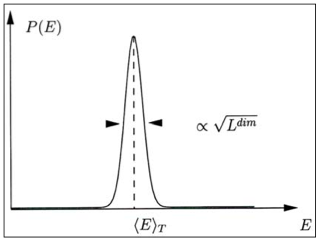
\includegraphics[width=0.5\textwidth]{pics/sampling}
		\label{fig:sampling}
  	\end{center}
  	\caption{Example of energy distribution}
\end{wrapfigure}

Often, choosing equally distributed configurations will be very inefficient since most of the possible configurations are unlikely to be assumed by the system. As an example take the kinetic energy of a gas. The distribution of the average energy will be a sharp peak, as in Fig. \ref{fig:sampling}. There are a number of methods to avoid unnecessary sampling of regions where the system is unlikely to be found (see \emph{importance sampling} in \citet{comp_phys} as an example). 

\end{comment}


A common way to choose the configurations to sample is introducing a virtual time $\tau$ and explore the phase space through a \emph{Markov chain}. Mind that the time $\tau$ has no physical meaning, and it only represents the steps of a stochastic process. 

In terms of a Markov chain, the transition probability from one state to another is given by the probability of a new state to be proposed ($T$) and the probability of this state to be accepted and assumed ($A$). In other words, $T(X\rightarrow Y)$ simply gives us the probability that a new configuration $Y$ is proposed, starting from the configuration $X$. This must fulfill three conditions:
\begin{enumerate}
\item \emph{Ergodicity}: any configuration in the phase space must be reachable within a finite number of steps
\item \emph{Normalization}: $\sum_Y{T(X\rightarrow Y)} =1$
\item \emph{Reversibility}:  $T(X\rightarrow Y)= T(Y\rightarrow X)$
\end{enumerate}
Once a configuration is proposed, one can accept the new configuration with probability $A(X\rightarrow Y)$ or reject it with probability $1- A(X\rightarrow Y)$. The transition probability is then given by
\begin{equation}
W(X\rightarrow Y) = T(X\rightarrow Y) \cdot A(X\rightarrow Y). 
\end{equation}
With the transition probability one can investigate the probability of finding the state in a certain configuration (during the stochastic process, not in real time!) $p\kl{X,\tau}$. The \emph{master equation} describes how the distribution evolves in time. 
\begin{equation}
\der{p\kl{X,\tau}}{\tau}=\sum_Y{p(Y)W(Y\rightarrow X)}  -\sum_Y{p(X)W(X\rightarrow Y) }
\label{eq:master}
\end{equation}
For Markov chains, it is known that the system always reaches a stationary state (called $p_{\text{st}}$) defined by the derivative in Eq. \eqref{eq:master} being zero. The transition probability must fulfill
\begin{enumerate}
\item \emph{Ergodicity}: any configuration must be reachable: $\forall X,Y:$ $W(X\rightarrow Y)\ge0$
\item \emph{Normalization}: $\sum_Y{W(X\rightarrow Y)} =1$
\item \emph{Homogeneity}:  $\sum_Yp_{\text{st}}(Y)W(Y\rightarrow X)= p_{\text{st}}(X)$
\end{enumerate} 
 
Note that the condition of reversibility is not required anymore. This is one of the effects of introducing $A\kl{X\rightarrow Y}$. Just think of a two level system, in which one of the two energy levels is higher (e.g. the electronic shells in an atom): At low energies it would be nonsense to equally sample the excited and the ground state of the electrons. On the contrary, at very high energies the sampling will have to reflect the higher probability of being in an excited state, rather then in the ground state. In order for the Markov chain algorithm to choose effectively which areas of the phase space to explore, somehow $W$ has to depend on the system. Imposing the distribution of the stationary states $p_\text{st}$ as the equilibrium distribution of the physical system $p_\text{st}$ (a real and measurable distribution) is called \emph{detailed balance}:
\begin{equation}
\der{p\kl{X,\tau}}{\tau}=0 \Leftrightarrow p_{\text{st}} \overset{!}{=}  p_{\text{eq}}
\label{eq:detailed_balance}
\end{equation}
It then follows from the stationary state condition ($\der{p\kl{X,\tau}}{\tau}=0$) that
$$\sum_Y{p_{\text{eq}}(Y)W(Y\rightarrow X)}  = \sum_Y{p_{\text{eq}}(X)W(X\rightarrow Y)}.$$ 
A sufficient (not necessary!) condition for this to be true is
 \begin{equation}
 {p_{\text{eq}}(Y)W(Y\rightarrow X)}  = {p_{\text{eq}}(X)W(X\rightarrow Y)}.
 \label{eq:detailed_balance2}
 \end{equation}
As an example, in a canonical ensemble (at fixed Temperature T), the equilibrium distribution is given by the Boltzmann factor: $p_{	\text{eq}}(X)= \frac{1}{Z_T}\text{exp}\ekl{-\frac{E(X)}{k_BT}}$ with the partition function $Z_T=\sum_X{ \text{exp}\ekl{-\frac{E(X)}{k_BT}} }$. The Boltzmann equilibrium indeed fulfills the detailed balance (see M(RT)$^2$ algorithm).




\subsubsection*{M(RT)$^2$ algorithm:}

If equation \eqref{eq:detailed_balance2} is fulfilled, we automatically found the way to fulfill detailed balance by the chosen $W$ and $p_{	\text{eq}}$. The algorithm (also called Metropolis algorithm\footnote{The rather curious name of this algorithm finds its reason in the names of the authors of the paper in which it was proposed: \citet{mrtrt}. \emph{RT} is squared because besides Metropolis, the other four authors of the paper formed two married couples and therefore carried the same family names. The real contributions of some of the authors (in particular of Metropolis and of A.H. Teller) is subject of controversy \citep{controversymrtrt,controversymrtrt2}. It has been even stated by Roy Glauber and Emilio Segr\'e that the original algorithm was invented by Enrico Fermi, which described it to Metropolis while they were working together at Los Alamos and later reinvented by Stan Ulam \citep{segre}.}) uses the acceptance probability 
\begin{equation}
A\kl{X\rightarrow Y} = min\ekl{1,\frac{p_{	\text{eq}}\kl{Y}}{p_{	\text{eq}}\kl{X}}}.
\label{eq:metropolis}
\end{equation}
In the case of the canonical ensemble with $p_{	\text{eq}}\kl{X} = \frac{1}{Z_T}\text{exp}\ekl{-\frac{E(X)}{k_BT}} $ the acceptance probability becomes then
\begin{equation}
A\kl{X\rightarrow Y} = min\ekl{1,\text{exp}\ekl{-\frac{E(Y)-E(X)}{k_BT}} }=min\ekl{1,\text{exp}\ekl{-\frac{\Delta E}{k_BT}} },
\end{equation}
which means that if the energy decreases, the step is always accepted, and if the energy increases it is accepted with probability $\text{exp}\ekl{-\frac{\Delta E}{k_BT}}$. Plugging Eq. \eqref{eq:metropolis} with $p_{	\text{eq}}$ into Eq. \eqref{eq:detailed_balance2} shows that detailed balance is fulfilled. For a more detailed discussion about the Metropolis and alternatives algorithms (e.g. Glauber dynamics), see \citet{comp_phys}. The algorithm has been then generalized in 1970 \citep{mrtrtgeneral}.
We can use this rather general algorithm to explore the phase space of the Ising model, by flipping the values on the lattice following the acceptance probability. Summarized, the steps in the Metropolis algorithm would then be:

\begin{itemize}
\item Choose (randomly) a site $i$
\item Calculate $\Delta E=E(Y)-E(X)=2J\sigma_i h_i$
\item If $\Delta E\leq0$, flip the spin, otherwise accept it with probability $\text{exp}\ekl{-\frac{\Delta E}{k_BT}}$
\end{itemize}
with $h_i=\sum_{i,j:nn}{\sigma_j}$ and $E=-J\sum_{i,j:nn}{\sigma_i\sigma_j}$. Mind that in the case of a squared lattice there are a limited number of possibilities that can occur. Consider creating a look-up table to spare computation time during the acceptance loop. For a 2D lattice, $h_i \in \mkl{0, \pm 2, \pm 4}$.
 
 
 \subsubsection*{Heat bath method (Glauber dynamics):}
The Metropolis algorithm is not the only possible Monte Carlo update: there are a number of other algorithms that fulfill Eq. \eqref{eq:detailed_balance2}. One of these has been elaborated by Glauber, with the acceptance probability given as

 \begin{equation}
A\kl{X\rightarrow Y} \equiv \frac{ \text{exp}\ekl{ - \frac{\Delta E}{k_B T} }}  {    1 + \text{exp}\ekl{ - \frac{\Delta E}{k_B T}}     }
\label{eq:glauber}
\end{equation}

One can see that the expression in Eq. \eqref{eq:glauber} fulfills Eq. \eqref{eq:detailed_balance2}:
 
 
 \begin{align*}
1 &= 1 \\
\Leftrightarrow  \frac{ 1 + \text{exp}\ekl{ - \frac{\Delta E}{k_B T} }  }  {    1 + \text{exp}\ekl{ - \frac{\Delta E}{k_B T}} } &= \text{exp}\ekl{ -\frac{\Delta E}{k_B T} }   \text{exp}\ekl{ +\frac{\Delta E}{k_B T} }  \\
\Leftrightarrow    \frac{ \kl{1 + \text{exp}\ekl{ +\frac{\Delta E}{k_B T}} }\text{exp}\ekl{ - \frac{\Delta E}{k_B T} }}  {    1 + \text{exp}\ekl{ - \frac{\Delta E}{k_B T}}     }  &= \text{exp}\ekl{\frac{ E_X-E_Y}{k_B T} }   \text{exp}\ekl{ +\frac{\Delta E}{k_B T} }   \\
\Leftrightarrow    \kl{1 + \text{exp}\ekl{ +\frac{\Delta E}{k_B T}} }\frac{ \text{exp}\ekl{ - \frac{\Delta E}{k_B T} }}  {    1 + \text{exp}\ekl{ - \frac{\Delta E}{k_B T}}     }  &= \frac{\text{exp}\ekl{\frac{ E_X}{k_B T} }}{\text{exp}\ekl{ \frac{E_Y}{k_B T} } }     \text{exp}\ekl{ +\frac{\Delta E}{k_B T} }   \\
\Leftrightarrow  \text{exp}\ekl{ \frac{E_Y}{k_B T} }    \frac{ \text{exp}\ekl{ - \frac{\Delta E}{k_B T} }}  {    1 + \text{exp}\ekl{ - \frac{\Delta E}{k_B T}}     }  &= \text{exp}\ekl{\frac{ E_X}{k_B T} }    \frac{ \text{exp}\ekl{ +\frac{\Delta E}{k_B T} }}  {    1 + \text{exp}\ekl{ +\frac{\Delta E}{k_B T}}     } \\
\underset{\text{const. temperature}}{\overset{T(X\rightarrow Y)\text{ symmetric}}{\Leftrightarrow}}  {p_{\text{eq}}(Y)T(Y\rightarrow X) A_{Gl.}(Y\rightarrow X)}  &= {p_{	\text{eq}}(X)T(X\rightarrow Y) A_{Gl.}(X\rightarrow Y)}.
\end{align*}
 
 


 
\noindent 
Mind that knowledge about the whole system configuration before the spin flip is not needed here: only the local configuration around the site is relevant. With $J = 1$, the probability to flip the spin $\sigma_i$ is:
$$
A_i = \frac{\text{exp}\ekl{\frac{-2 \sigma_i h_i}{k_BT}}}{1+\text{exp}\ekl{\frac{-2 \sigma_i h_i}{k_BT}}}
$$
with $h_i$ being the local field as usual $h_i = \sum_{j=nn}{\sigma_j}$. Using the abbreviation $p_i \equiv \frac{\text{exp}\ekl{2 \beta h_i}}{1+\text{exp}\ekl{2 \beta h_i}}$, one can express the probability to flip the spin as being

\begin{equation}
p_{\text{flip}} =\begin{cases}
  p_i  & \text{for }\sigma_i=-1\\
  1-p_i & \text{for }\sigma_i=+1
\end{cases}
\text{\hspace{0.5cm} and  \hspace{0.5cm}}\hfill 
p_{\text{no flip}}   =\begin{cases}
  1- p_i  & \text{for }\sigma_i=-1\\
  p_i & \text{for }\sigma_i=+1
\end{cases}
\end{equation}

\noindent
This can be implemented as  $$\sigma_i(\tau+1)=-\sigma_i(\tau)\cdot sign(A_i-z),$$ with $z$ being a random number, or as
$$
\sigma_i(\tau+1) = \begin{cases}
  +1  & \text{with propability }p_i\\
  -1 & \text{with propability }1- p_i
\end{cases}
\text{\hspace{0.5cm} with  \hspace{0.5cm}}\hfill 
p_i \equiv \frac{\text{exp}\ekl{2 \beta h_i}}{1+\text{exp}\ekl{2 \beta h_i}}
$$

This method which does not depend on the spin at time $t$, is called \emph{heat bath MC}.


 
 
\subsubsection*{Binary mixtures (Kawasaki dynamics):}
In this method, the sum of the spins pointing up and the sum of the spins pointing down (i.e., the magnetization) is held constant. Kawasaki dynamics can be used for simulating  binary mixtures of gases and other systems were the population numbers are conserved. In the case of a two species mixture, the energy is larger for A-B bonds, with A and B being the two species in the binary mixture (spin up and spin down particles, two different gas molecules, etc.). What  one can do is to switch two particles with a certain probability and then add the configuration to the averaging loop. 

\subsubsection*{Creutz algorithm:}
Let us consider a situation in which energy is constant. The algorithm generally used in this case is the \emph{Creutz} algorithm. In this technique the condition of energy conservation is relaxed a bit and energy is not exactly conserved anymore. The movement in phase space is therefore not strictly constrained to a subspace of constant energy, but we have a certain additional volume in which we can freely move. The condition is softened by introducing a \emph{demon}, which is a small reservoir of energy $E_d$ that can store a certain maximum energy $E_m$:

\begin{itemize}
\item Choose a site
\item Calculate $\Delta E$ for the spin flip
\item Accept the change if $E_m\ge E_d-\Delta E\ge 0 $
\end{itemize}
This method is completely deterministic (besides the fact that one can randomly choose the sites to update) and therefore reversible. The drawback is that the temperature of the system is not known, but it can be estimated  with the Boltzmann distribution. Taking a histogram of the energies $E_d$ one observes a distribution $P(E_d)\propto \text{exp}\ekl{ -\frac{E_d}{k_BT} }$. The fit is not optimal, since one has very few values of $E_d$. The bigger $E_m$, the faster is the method, since the condition of constant energy is relaxed and the exploration of phase space is less restricted to certain regions. 



\subsubsection*{Q2R:}
In the case of $E_m\rightarrow0$, the Creutz algorithm becomes a totalistic cellular automaton called \emph{Q2R}. The update rules on a square lattice are then given by
 $$
 \sigma_{i,j}(\tau+1) = f(x_{ij})\oplus\sigma_{i,j}(\tau)
 $$
with 
$$
x_{i,j}= \sigma_{i-1,j} +\sigma_{i+1,j} +\sigma_{i,j-1} +\sigma_{i,j+1}
\text{\hspace{0.5cm} and  \hspace{0.5cm}}\hfill 
f(x)=\begin{cases}
  1  & \text{if }x=2\\
  0 & \text{if }x\neq 2
\end{cases}
$$
In this case, the spins are flipped if and only if the change in energy is zero. This can be implemented in a very efficient way using multi spin coding. The changer word defined by $f(x)$ can be expressed in a very elegant way using logical functions:
$$
\sigma(\tau+1) = \sigma(\tau)\oplus\mkl  { \ekl{\kl{\sigma_1\oplus \sigma_2}  \wedge  \kl{\sigma_3\oplus \sigma_4} }  \lor   \ekl{\kl{\sigma_1\oplus \sigma_3}  \wedge  \kl{\sigma_2\oplus \sigma_4} } }
$$
This logical expression can be computed in roughly 12 cycles (8 logical operation and 4 fetches) which last typically around $10$ns. At this computational speed and using multi spin coding (see Sec. \ref{sec:multi_spin}) one can roughly update 4 sites per nanosecond. The method is extremely fast, deterministic and reversible. The problem is that it is not ergodic, and that it strongly depends on the initial configuration. As an example, try to imagine the development of a small lattice, in which only $\sigma_{2,1}$ and $\sigma_{1,2}$ are equal to +1. In fact, this method is not used in statistical physics but it is useful for other purposes e.g., neuroinformatics or cellular automata.




 \subsection{Boundary conditions:}
 
When simulating a lattice, one of the finite size effects that one has to take into account is that at the boundaries the sites do not have further neighbors. The values there can be fixed (boundary condition) or periodic boundaries can be introduced. Mind that this is not only a question of finite size effects, but it can also correspond to some real physical situation. As an example, think of some zero potential boundary condition while solving the electrostatic potential using finite difference methods\footnote{See \citet{comp_phys}}. In finite lattices following methods can be used:

\begin{itemize}
\item Open boundaries, i.e. no neighbors at the edges of the system.
\item Fixed boundary conditions,
\item and periodic boundaries.
\end{itemize}

If our system is big enough\footnote{\emph{Big} here is not purely arbitrary but it depends on what we want to simulate. A good measure of \emph{big} can be that the edges of the system are uncorrelated. It is clear that this method is useless in \emph{small} lattices.} one identies the two sides of the lattice as being neighbors. ($\sigma_{i,L+1}\equiv\sigma_{i,1}$, and $\sigma_{L+1,j}\equiv\sigma_{1,j}$). Identifying the last element of a row (or column) with the first element of the next row (or column) leads to so called \emph{helical boundary condition}. $\sigma_{i,L+1}\equiv\sigma_{i+1,1}$, therefore one can use only one index $k = i+j(L-1)$ instead of keeping track of two.



\subsection{Sampling Uncorrelated Configurations}
Each time we accept a spin-flip in our sampling chain, a new configuration is generated. The problem is that the new and the previous configurations are strongly correlated, and the error analysis (e.g., the decreasing of the error like $\propto \frac{1}{\sqrt{N}}$) is no longer valid. We have to find a measure to know whether we already are in equilibrium or not and to be sure that we are sampling uncorrelated configurations. The (Monte Carlo) time evolution of a quantity is defined as

\begin{equation}
\avkl{A(\tau)}= \sum_X{p\kl{X,\tau}A\kl{X\kl{\tau}}} \overset{\text{eq.}}{=} \sum_X{p\kl{X,\tau_0}A\kl{X(\tau)}}
\end{equation} 




\vspace{0.1cm}
\noindent
\begin{minipage}{\textwidth}
\begin{minipage}{.48\textwidth}

With the condition expressed in \eqref{eq:master}, we know how the probability distribution $p$ evolves. If we assume that our configuration distribution is not at equilibrium at $\tau = \tau_0$, we can define the \emph{non-linear correlation function}:
\begin{equation}
\Phi_A^{nl}\kl{\tau} = \frac {\avkl{A(\tau)}- \avkl{A(\infty)}}  {\avkl{A(\tau_0)}- \avkl{A(\infty)}}
\end{equation}
This is not a correlation function in the strict sense, but it can be a measure to investigate the correlation of the configurations. 
\end{minipage}%
\hfill
\begin{minipage}{.48\textwidth}
  \centering
  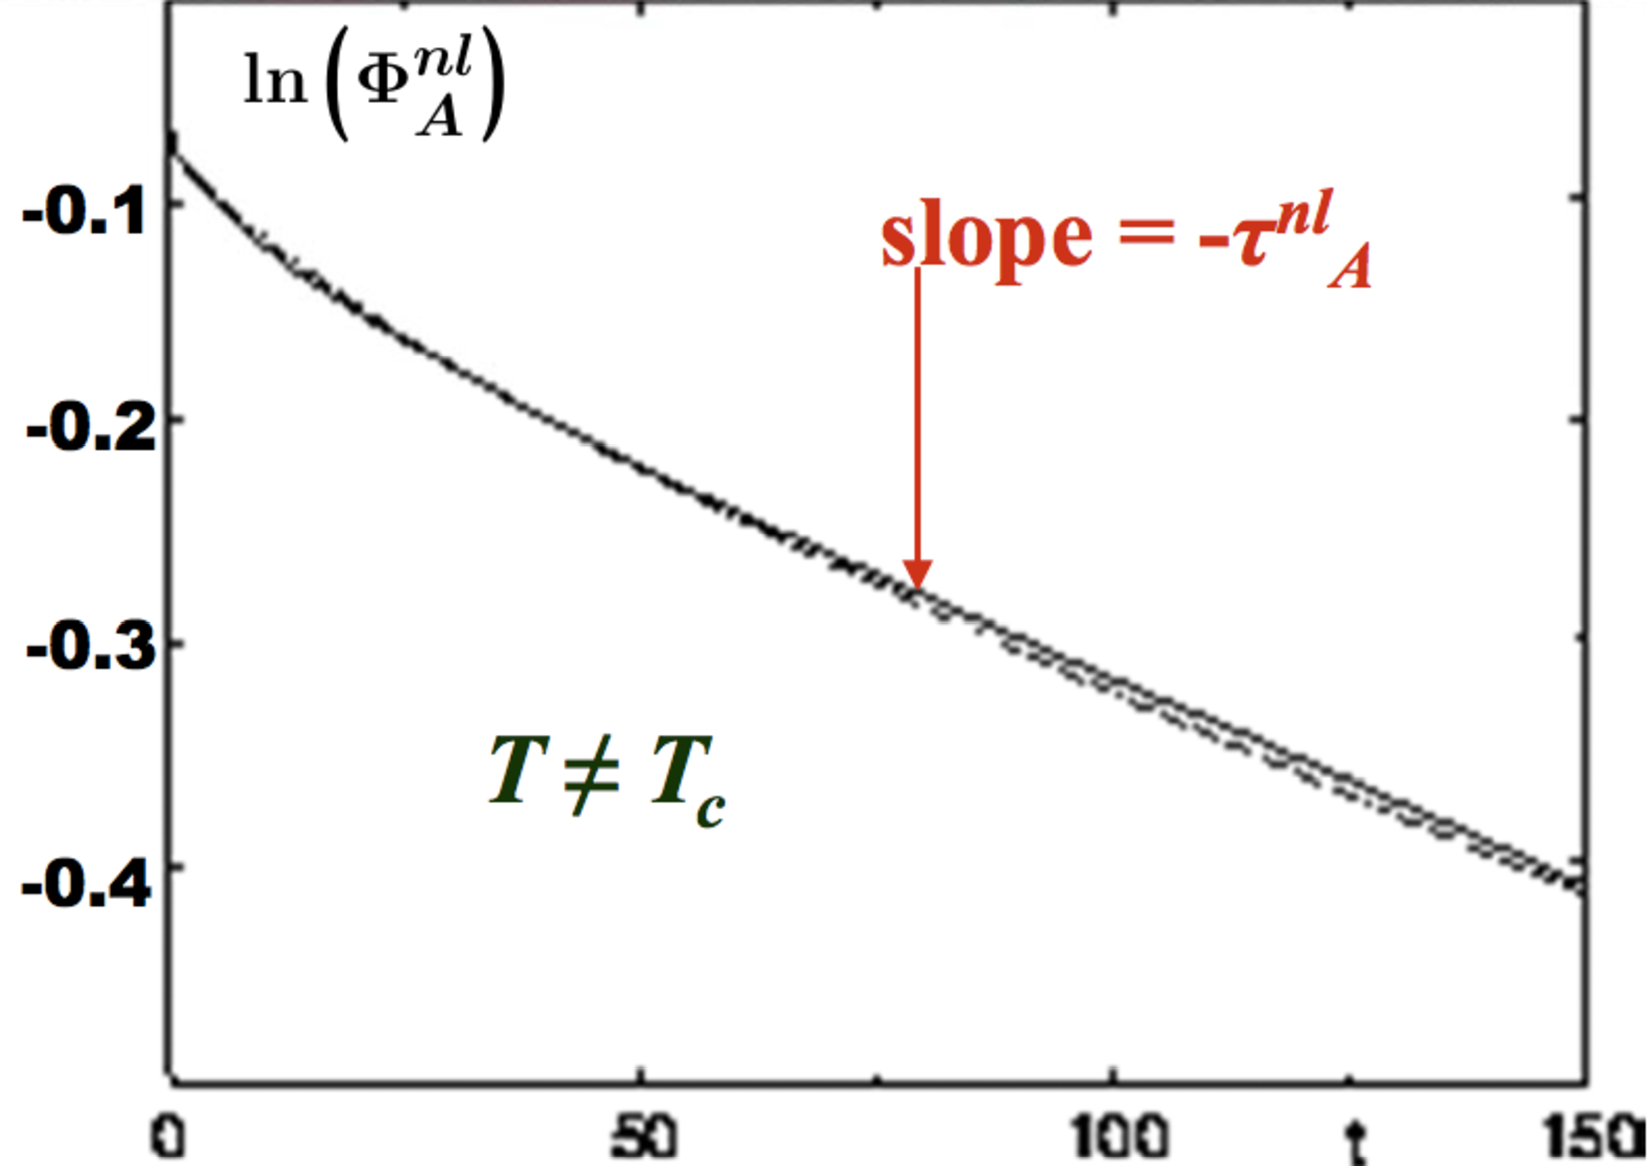
\includegraphics[height=150pt]{pics/non_lin_corr_fun}
  \captionof{figure}{Non-linear correlation function over Monte Carlo time.}
  \label{fig:non_lin_corr_fun.pdf}
\end{minipage}
\end{minipage}
\vspace{0.1cm}



The \emph{non-linear} correlation time $\tau_A^{nl}$ describes the relaxation towards equilibrium:
\begin{equation}
\tau_A^{nl} \equiv \int_0^{\infty} \Phi_A^{nl}\kl{\tau} d\tau
\end{equation}
Near $T_c$, it assumes the form of a power law (\emph{critical slowing down}):
\begin{equation}
\tau_A^{nl} \propto \abs{T-T_c}^{-z_A^{nl}}
\end{equation} with $z_A^{nl}$ being the non-linear dynamical critical exponent. This means that at $T_c$, the time needed to reach equilibrium diverges!






The linear correlation function of two values $A$, $B$
\begin{equation}
\Phi_{AB}\kl{\tau} = \frac {\avkl{A(\tau_0)B(\tau)}- \avkl{A}\avkl{B}}  {\avkl{A B}- \avkl{A}\avkl{B}}
\label{eq:lin_corr_fun}
\end{equation} with $$ \avkl{A\kl{\tau_0} B\kl{\tau}}     =  \sum_X{   p\kl{X,\tau_0} A\kl{X\kl{\tau_0}} B \kl{X\kl{\tau}}     }$$
is now a proper correlation function. Note that it goes from 1 to 0 when $\tau$ goes to infinity. If $A=B$, we call Eq. \eqref{eq:lin_corr_fun} the \emph{autocorrelation function}. For the spin-spin correlation in the Ising model we get:

$$\Phi_{\sigma}\kl{\tau} = \frac {\avkl{\sigma(\tau_0)\sigma(\tau)}- \avkl{\sigma(\tau_0)}^2} {\avkl{\sigma^2(\tau_0)}- \avkl{\sigma(\tau_0)}^2}$$

The \emph{linear} correlation time $\tau_A^{nl}$ describes the relaxation in equilibrium:
\begin{equation}
\tau_{AB} \equiv \int_0^{\infty} \Phi_{AB}\kl{\tau} d\tau
\end{equation}

  \begin{center}
  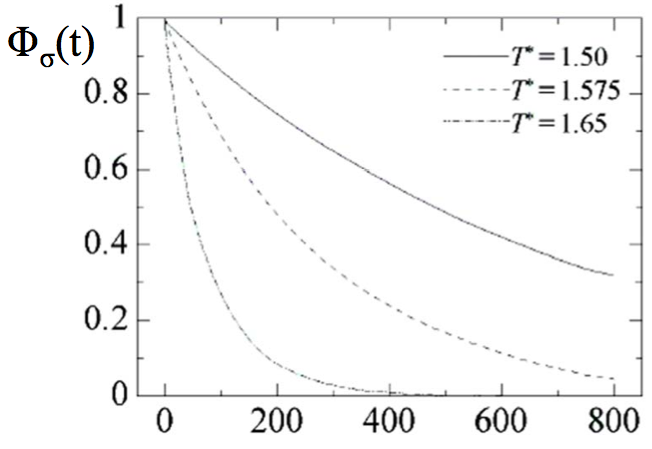
\includegraphics[width=0.7\textwidth]{pics/spin_spin_fun}
  \captionof{figure}{Spin-spin autocorrelation function over MC time in the Ising model.}
  \label{fig:spin_spin_fun}
\end{center}

\begin{comment}

\vspace{0.1cm}
\noindent
\begin{minipage}{\textwidth}
\begin{minipage}{.48\textwidth}
\noindent
If $A=B$, we call Eq. \eqref{eq:lin_corr_fun} the \emph{autocorrelation function}. For the spin-spin correlation in the Ising model we get:

$$\Phi_{\sigma}\kl{\tau} = \frac {\avkl{\sigma(\tau_0)\sigma(\tau)}- \avkl{\sigma(\tau_0)}^2} {\avkl{\sigma^2(\tau_0)}- \avkl{\sigma(\tau_0)}^2}$$

\end{minipage}%
\hfill
\begin{minipage}{.48\textwidth}
  \centering
  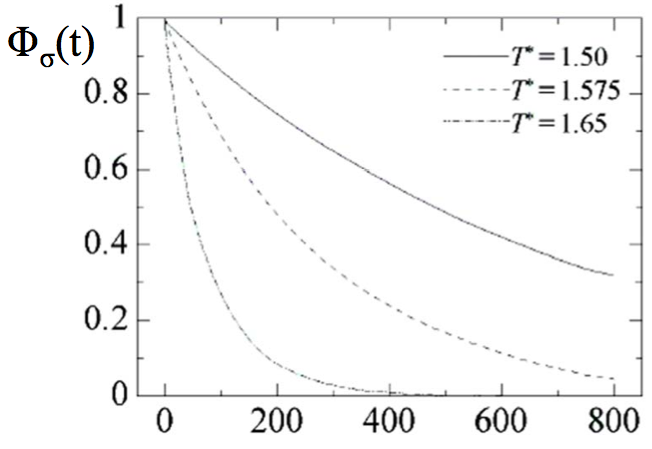
\includegraphics[height=150pt]{pics/spin_spin_fun}
  \captionof{figure}{Spin-spin autocorrelation function over MC time in the Ising model.}
  \label{fig:spin_spin_fun}
\end{minipage}
\end{minipage}
\vspace{0.1cm}

\end{comment}



Near $T_c$, it assumes the form of a power law (\emph{critical slowing down}):
\begin{equation}
\tau_{AB} \propto \abs{T-T_c}^{-z_A}
\end{equation} with $z_A$ being the \emph{linear} dynamical critical exponent.




The dynamical exponents turn out to be 
$$z_\sigma = 2.16 \text{ (in 2D)}$$ $$z_\sigma = 2.09 \text{ (in 3D)}$$ There is a conjectured relation between the critical exponents of the previous sections and the critical dynamical exponents (for spin and for energy correlation) that is numerically well established but not yet analytically proven:

\begin{align}
z_\sigma - z_\sigma^{nl} &= \beta \\ 
z_E - z_E^{nl} &=1- \alpha\\
\end{align}


\subsubsection*{Decorrelated configurations:}


\vspace{0.1cm}
\noindent
\begin{minipage}{\textwidth}
\begin{minipage}{.48\textwidth}
\noindent

The behavior we studied until now is only valid in the case of an infinite lattice. In a finite system there is no divergence by definition (See \citet{comp_phys}). The correlation length diverges at the critical temperature $T_c$:
\begin{equation}
L=\xi\kl{T}\propto \abs{T-T_c}^{-\nu}
\label{eq:corr_len_div}
\end{equation}
$$\Rightarrow \tau_{AB} \propto \abs{T-T_c}^{-z_{AB}}\propto L^{\frac{z_{AB}}{\nu}} $$ 
which means that with growing system size, the number of samples to be discarded also increases.


\end{minipage}%
\hfill
\begin{minipage}{.48\textwidth}
  \centering
  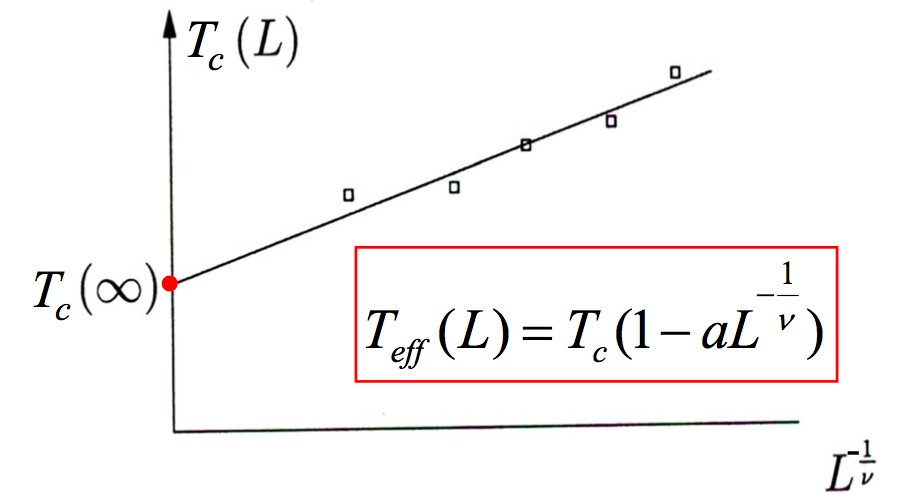
\includegraphics[height=150pt]{pics/finite_size}
  \captionof{figure}{Finite size effects for different system sizes can be used to obtain the critical temperature by extrapolation. See \citet{comp_phys}}
  \label{fig:finite_size}
\end{minipage}
\end{minipage}
\vspace{0.1cm}

\noindent
This is a problem when sampling big systems since the computation becomes very expensive. To be sure not to sample correlated configurations one should 
\begin{itemize}
\item reach equilibrium first  (discard $n_0 = c \tau^{nl}(T)$ configurations).
\item Sample every $n_e^{th}=c \tau(T)$ configurations.
\item At $T_c$ use $n_0 = c L^{\frac{z^{nl}}{\nu}}$ and $n_e=c L^{\frac{z}{\nu}}$
\end{itemize}
where $c \approx 3$ is a "safety factor" to make be sure to discard enough samples. A trick for reducing this effect is using cluster algorithms, which we will encounter later on.

